\section{Reinfocement Learning}
\label{sect:reinforcement-learning}
\begin{itemize}
	\item agent can act
	\item actions change the agent's future state
	\item scalar rewards for success
	\item (sequential decision making
\end{itemize}
\textit{Select actions to maximize the future reward}.\\
Examples of Reinforcement Learning:
\begin{itemize}
	\item Fly stunt maneuver in a	 helicopter
	\item Defeat the world champion at backgammon	
	\item Manage an investment portfolio
	\item Control a power station
	\item Make a humanoid robot walk
	\item Play many different Atari games better than humans	
\end{itemize}
\begin{figure}[h]
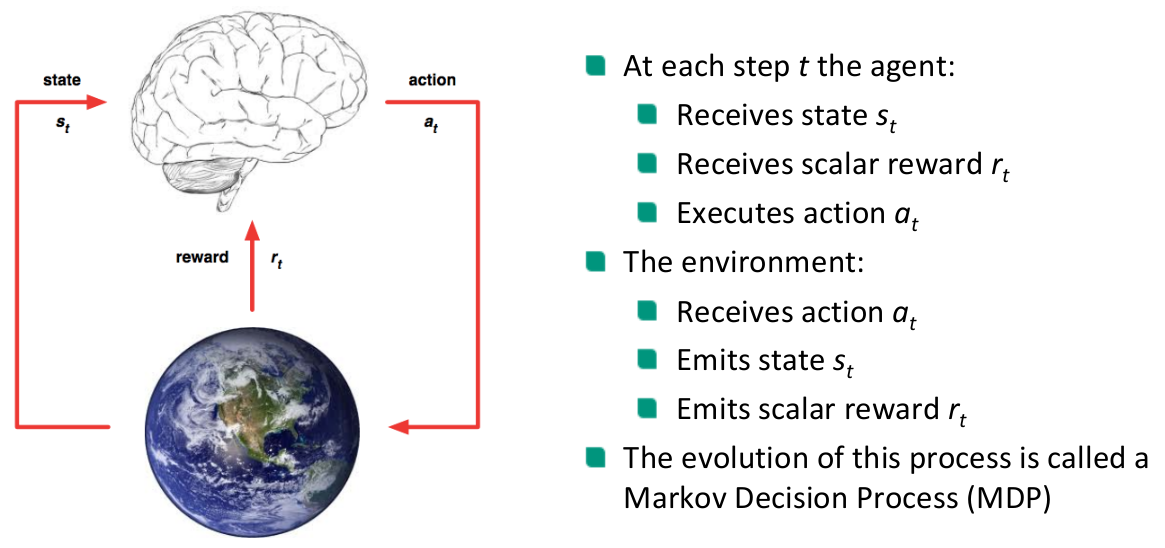
\includegraphics[scale=0.4]{agent-and-environment}
\end{figure}
\textbf{Policy} $a = \pi(s)$: probabilty distribution of actions given a state\\
\textbf{Value function} $Q^{\pi}(s, a)$: expected total reward from state $s$ and action $a$ under policy $\pi$
\[
Q^{\pi}(s, a) = \mathbb{E}[r_{t + 1} + \gamma r_{t + 2} + \gamma^2 r_{t + 2} + \gamma^3 r_{t + 3} + ... | s, a]
\]
\textbf{Policy-based RL}: search directly for the optimal policy $\pi$ (achieving maximum future reward)\\
\textbf{Value-based RL}: estimate optimal value function $Q^*(s, a)$ (maximum value achievable under any policy)\\
To train these networks we use \textit{Monte Carlo methods} to learn from experience.
\textbf{Policy-based Reinforcement Learning}: parameterize the policy (for example with a neural network) and based on the cumulative rewards, update the policy. We need to get the gradient of the rewards with respect to the policy:
\begin{itemize}
	\item Policy Gradients algorithm
	\item Online: update after episode
	\item Offline: update while in episodes
\end{itemize}
\begin{figure}[h]
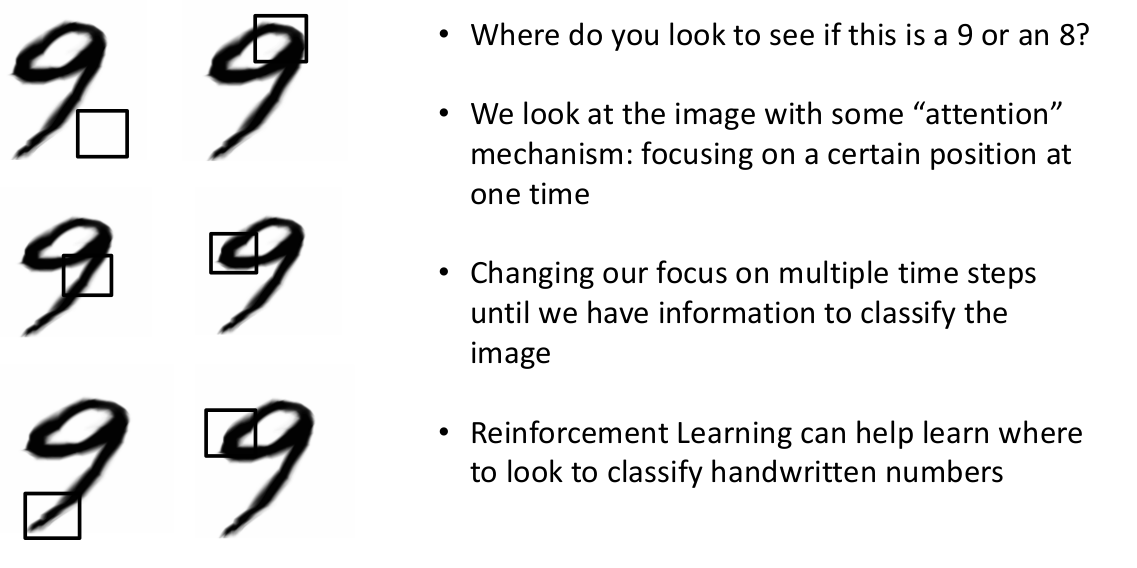
\includegraphics[scale=0.4]{policy-gradients-with-neural-networks}
\end{figure}
For the image shown we can use a RNN to determine what our current state is given the last state. RL for where should we look next, given our current states.
\begin{figure}[h]
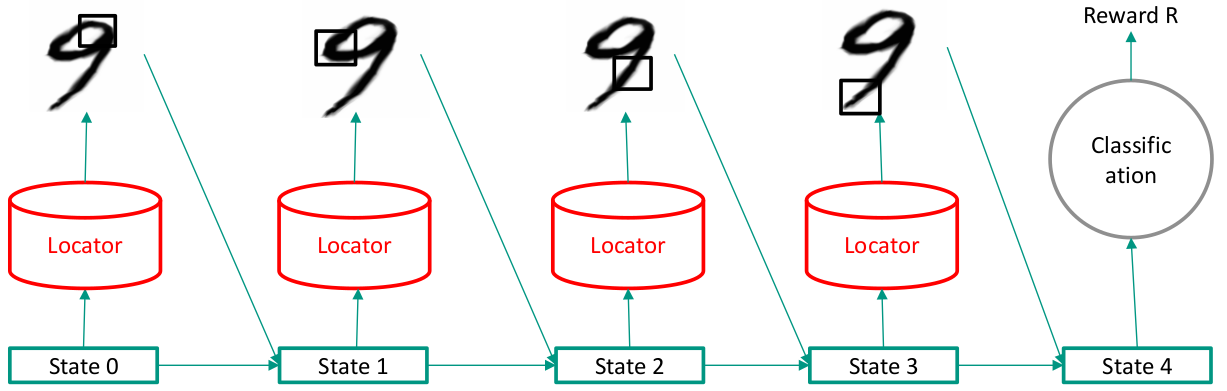
\includegraphics[scale=0.4]{RL-rrn-rl}
\end{figure} \\
RL gives use an reward on which we can calculate the backward pass (reward represents the gradient).
\begin{figure}[h]
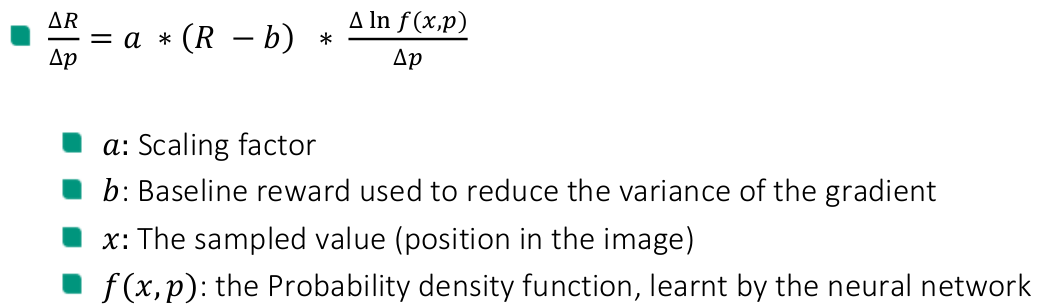
\includegraphics[scale=0.4]{policy-gradient-with-neural-networks}
\end{figure}\\[2cm]

\subsection{Bellman Equation}
\label{ssect:bellman-equation}
\[
Q^{\pi}(s, a) = \mathbb{E}[r_{t + 1} + \gamma r_{t + 2} + \gamma^2 r_{t + 2} + \gamma^3 r_{t + 3} + ... | s, a]
\]
Recursively:
\[
Q^{\pi}(s, a) = \mathbb{E}_{s^{'}}[r_{t + 1} + \gamma Q^{\pi}(s^{'}, a^{'})| s, a]
\]
Optimal value function:
\[
Q^{*}(s, a) = \mathbb{E}_{s^{'}}[r_{t + 1} + \gamma Q^{\pi}(s^{'}, a^{'})| s, a]
\]
Value iteration solve the Ballman Equation:
\[
Q_{i + 1}(s, a) = \mathbb{E}_{s^{'}}[r_{t + 1} + \gamma Q_i(s^{'}, a^{'})| s, a]
\]


\newpage